\chapter{作物模式}
%\addcontentsline{toc}{chapter}{作物模式}
\begin{mymdframed}{代码}
  本章对应代码源文件位于\texttt{main/BGC/}目录下。
\end{mymdframed}

%\begin{作物模式}
GPAM1可以模拟作物生长发育的关键过程及其对天气/气候、近地面大气$\mathrm{CO_2}$和$\mathrm{O_3}$浓度和氮沉降、
农田管理的响应和生物、化学、物理反馈。
下面详述作物区别于自然植被、需要特殊处理的过程参数化方案。

GPAM1包含64个作物功能类型(Crop Functional Type, CFT)(表~\ref{tab:CoLM预设作物功能类型}),但目前可打开使用的是14个,模拟5种作物类型: 冬小麦、春小麦、水稻、玉米、大豆(图~\ref{fig:作物功能类型覆盖率的空间分布})。每种作物类型各分雨养(rainfed)和灌溉(irrigated)CFT,玉米和大豆又分温带和热带。每个CFT占用一个水热独立的陆表单元(patch)。
{
  \begin{table}[htbp]
    \centering
    \caption{CoLM里预设的作物功能类型(CFT)及目前打开可模拟的CFT}
    \label{tab:CoLM预设作物功能类型}
    \begin{tabular}{@{}clc|clc@{}}
      \toprule
      Index & CFT名称            & 打开?     & Index & CFT名称      & 打开?     \\
      \midrule
      15    & 无管理的雨养C3作物 &            & 47    & 雨养葡萄     &            \\
      16    & 无管理的灌溉C3作物 &            & 48    & 灌溉葡萄     &            \\
      17    & 温带雨养玉米       & \checkmark & 49    & 雨养花生     &            \\
      18    & 温带灌溉玉米       & \checkmark & 50    & 灌溉花生     &            \\
      19    & 雨养春小麦         & \checkmark & 51    & 雨养小米     &            \\
      20    & 灌溉春小麦         & \checkmark & 52    & 灌溉小米     &            \\
      21    & 雨养冬小麦         & \checkmark & 53    & 雨养油棕     &            \\
      22    & 灌溉冬小麦         & \checkmark & 54    & 灌溉油棕     &            \\
      23    & 温带雨养大豆       & \checkmark & 55    & 雨养马铃薯   &            \\
      24    & 温带灌溉大豆       & \checkmark & 56    & 灌溉马铃薯   &            \\
      25    & 雨养大麦           &            & 57    & 雨养豆类     &            \\
      26    & 灌溉大麦           &            & 58    & 灌溉豆类     &            \\
      27    & 雨养冬大麦         &            & 59    & 雨养油菜籽   &            \\
      28    & 灌溉冬大麦         &            & 60    & 灌溉油菜籽   &            \\
      29    & 雨养黑麦           &            & 61    & 雨养水稻     & \checkmark \\
      30    & 灌溉黑麦           &            & 62    & 灌溉水稻     & \checkmark \\
      31    & 雨养冬黑麦         &            & 63    & 雨养高粱     &            \\
      32    & 灌溉冬黑麦         &            & 64    & 灌溉高粱     &            \\
      33    & 雨养木薯           &            & 65    & 雨养甜菜     &            \\
      34    & 灌溉木薯           &            & 66    & 灌溉甜菜     &            \\
      35    & 雨养柑橘           &            & 67    & 雨养甘蔗     &            \\
      36    & 灌溉柑橘           &            & 68    & 灌溉甘蔗     &            \\
      37    & 雨养可可           &            & 69    & 雨养向日葵   &            \\
      38    & 灌溉可可           &            & 70    & 灌溉向日葵   &            \\
      39    & 雨养咖啡           &            & 71    & 雨养芒草     &            \\
      40    & 灌溉咖啡           &            & 72    & 灌溉芒草     &            \\
      41    & 雨养棉花           &            & 73    & 雨养柳枝稷   &            \\
      42    & 灌溉棉花           &            & 74    & 灌溉柳枝稷   &            \\
      43    & 雨养枣椰树         &            & 75    & 热带雨养玉米 & \checkmark \\
      44    & 灌溉枣椰树         &            & 76    & 热带灌溉玉米 & \checkmark \\
      45    & 雨养牧草           &            & 77    & 热带雨养大豆 & \checkmark \\
      46    & 灌溉牧草           &            & 78    & 热带灌溉大豆 & \checkmark \\
      \bottomrule
    \end{tabular}
  \end{table}
}

{
  \begin{figure}[htbp]
    \centering
    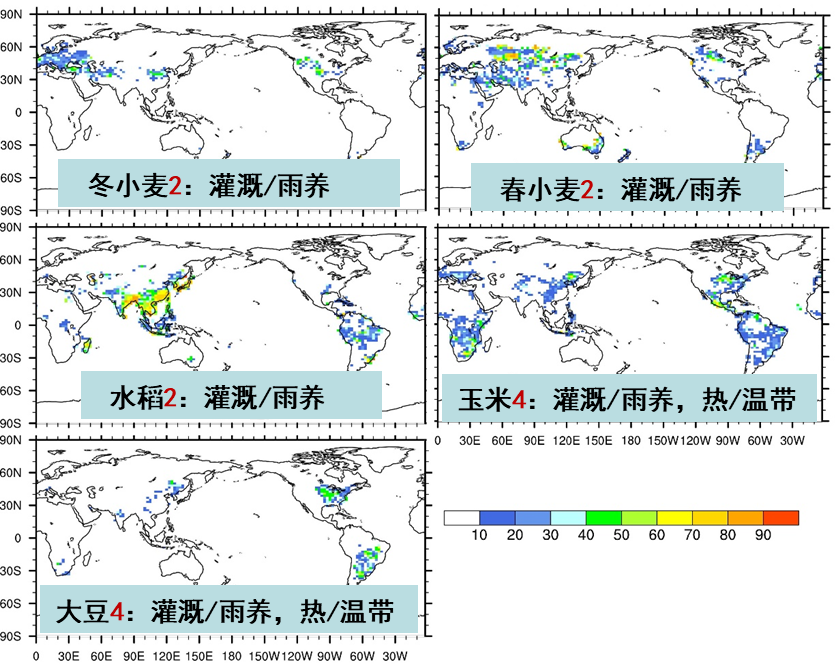
\includegraphics[scale=0.9]{Figures/作物模式/GPAM1模式模拟的14个作物功能类型格点面积覆盖率空间分布.png}
    \caption{GPAM1模式模拟的14个作物功能类型(CFT)格点面积覆盖率(\%)的空间分布}
    \label{fig:作物功能类型覆盖率的空间分布}
  \end{figure}
}

\section{物候}
GPAM1的物候包括三个阶段: (1)播种到抽芽; (2)抽芽到开始灌浆(grain fill); (3)灌浆到成熟/收割。所涉及的参数取值见表~\ref{tab:作物物候方案相关参数}。

% Please add the following required packages to your document preamble:
% \usepackage{booktabs}
\begin{table}[htbp]
  \centering
  \caption{作物物候方案相关参数}
  \label{tab:作物物候方案相关参数}
  \begin{tabular}{@{}cccccc@{}}
    \toprule
           & $T_{\mathrm{base}}$ & $f_{\mathrm{LE}}$ & $f_{\mathrm{GF}}$ & ${\rm GDD}_{\mathrm{mat}}$  & ${\rm GSL}_{\mathrm{max}}$ \\ \midrule
    春小麦 & 0                   & 0.07              & 0.60              & 0.2${\rm GDD}_{\rm 10yr}$+1458  & 150                  \\
    冬小麦 & 0                   & 0.03              & 0.67              & 0.38${\rm GDD}_{\rm 10yr}$+526  & 270                  \\
    水稻1  & 10                  & 0.12              & 0.68              & 0.30${\rm GDD}_{\rm 10yr}$+695  & 150                  \\
    水稻2  & 10                  & 0.35              & 0.75              & 0.27${\rm GDD}_{\rm 10yr}$+575  & 150                  \\
    玉米   & 8                   & 0.11              & 0.64              & 0.26${\rm GDD}_{\rm 10yr}$+907 & 150                  \\
    大豆   & 10                  & 0.15              & 0.69              & 0.26${\rm GDD}_{\rm 10yr}$+802  & 150                  \\ \bottomrule
  \end{tabular}
\end{table}

\subsection{播种}\label{sec:播种}
  播种日期是给定的,采用全球播种日再分析数据~\citep{jagermeyr2021climate}),并结合陆表数据中的作物分布制作而成 (图~\ref{fig:GPAM1播种日空间分布}),为GPAM1的输入场。

{
\begin{figure}[htbp]
  \centering
  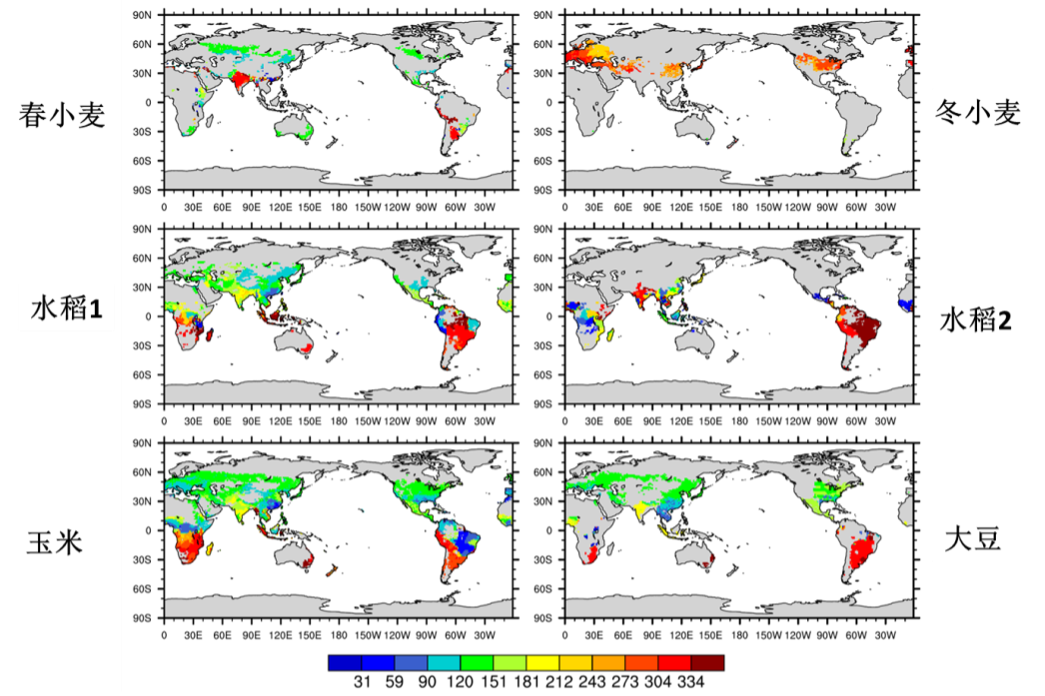
\includegraphics[scale=1.2]{Figures/作物模式/GPAM1播种日空间分布.png}
  \caption{GPAM1播种日空间分布}
  \label{fig:GPAM1播种日空间分布}
\end{figure}
}

\subsection{抽芽}
当热单元指数(Heat Unit Index, ${\mathrm {HUI}}$):
\begin{equation}\label{HUI}
  {\mathrm {HUI}}=\frac{{\rm GDD}_{\mathrm{base}}}{{\rm GDD}_{\mathrm{mat}}}
\end{equation}
达到$f_{\mathrm{LE}}$时,开始抽芽。${\rm GDD}_{\mathrm{base}}$是基于陆表气温的积温(\textcelsius\ days):
\begin{equation}
  {\rm GDD}_{\mathrm{ {base }}}=\sum_{\mathrm{planting}}^{\rm current\ day} \min \left(0, T_{\mathrm{sa}}-T_{\mathrm{base}}\right)
\end{equation}
其中,$T_{\mathrm{sa}}$是日地表气温\todo{需更加明确,与前面相同变量统一符号。},$T_{\mathrm{base}}$是底温(作物在该温度下停止生长)。

\subsection{灌浆}
当${\mathrm {HUI}}$达到$f_{\mathrm{GF}}$时,开始灌浆。

\subsection{成熟}
当${\mathrm {HUI}}$达到1时或生长季达到最长生长季长度${\rm GSL}_{\mathrm{max}}$时,作物成熟。其中,${\rm GDD}_{\mathrm{mat}}$是${\rm GDD}_{\mathrm{base}}$
10年滑动平均的一元线性方程(表~\ref{tab:作物物候方案相关参数})。
\begin{equation}
  {\rm GDD}_{\mathrm{mat}}=a {\rm GDD}_{\rm 10yr}+b
\end{equation}

\subsection{收割}
假设达到成熟的时步收割。


\section{生理变化}
作物的碳(C)库和氮(N)库有leaf, live stem, grain, fine root库及相应的transfer和storage库,无dead stem, live coarse root, dead coarse root库及相应的transfer和storage库。由于新加了grain库,相应通量会增加分配到grain的C/N通量,grain到Aproduct及litter的C/N通量。作物的呼吸和周转与草相同。

\subsection{光合和气孔导度}
大豆、小麦、水稻采用C3植物光合方案;玉米采用C4植物光合方案。
在基于Medlyn方案计算气孔导度时,玉米的参数取值$g_1=1.8$,低于自然植被,其余作物的参数取值$g_1=5.8$,高于自然植被。该参数越大,气孔导度越高。

\subsection{分配}
分配系数随物候阶段变化而变化。从出叶开始,按下列分配系数公式分配到叶库Cleaf,茎库Cleaf,根库Croot,粒库Cgrain。
不同物候期分配系数见表~\ref{tab:作物分配方案相关参数}。

(1)	物候期2 \\
\begin{equation}
  \left\{\begin{array}{c}
      a_{\mathrm{grain}}=0 \\
      a_{\mathrm{root}}=a_{\mathrm{root\_i}}-\left(a_{\mathrm{root\_i}}-a_{\mathrm{root\_f}}\right) {\mathrm {HUI}} \\
      a_{\mathrm{leaf}}=\left(1-a_{\mathrm{root}}\right) a_{\mathrm{leaf\_i}} \frac{{\rm e}^{-{b}}-{\rm e}^{-b \frac{{\mathrm {HUI}}}{f_{\mathrm{GF}}}}}{{\rm e}^{-{b}}-1}   \\
      a_{\mathrm{stem}}=1-a_{\mathrm{grain}}-a_{\mathrm{root}}-a_{\mathrm{leaf}}
  \end{array}\right.
\end{equation}
其中,下标$i$和$f$表示该分配系数的初值和终值,$b=0.1$。

(2)	物候期3 \\
\begin{equation}
  \left\{\begin{array}{c}
      a_{\mathrm{leaf}}=0.0 \\
      a_{\mathrm{root}}=a_{\mathrm{root\_i}}-\left(a_{\mathrm{root\_i}}-a_{\mathrm{root\_f}}\right) \min(1, {\mathrm {HUI}}) \\
      a_{\mathrm{stem}}=\max \left[a_{\mathrm{stem\_f}}, a_{\mathrm{stem}} \max \left(0, \frac{1-{\mathrm {HUI}}}{1-f_{\mathrm{GF}}}\right)^{d_{\mathrm{sem}}}\right] \\
      a_{\mathrm{grain}}=1-a_{\mathrm{root}}-a_{\mathrm{leaf}}-a_{\mathrm{stem}}
  \end{array}\right.
\end{equation}
% Please add the following required packages to your document preamble:
% \usepackage{booktabs}
\begin{table}[htbp]
  \centering
  \caption{作物分配方案相关参数}
  \label{tab:作物分配方案相关参数}
  \begin{tabular}{@{}lcccc@{}}
    \toprule
    参数                        & 小麦 & 水稻 & 玉米 & 大豆 \\ \midrule
    $\alpha_{\mathrm{leaf\_i}}$ & 0.9  & 0.75 & 0.8  & 0.85 \\
    $\alpha_{\mathrm{root\_i}}$ & 0.1  & 0.1  & 0.4  & 0.2  \\
    $\alpha_{\mathrm{root\_f}}$ & 0    & 0    & 0.05 & 0.2  \\
    $\alpha_{\mathrm{stem\_f}}$ & 0.05 & 0.05 & 0.0  & 0.3  \\
    $d_{\mathrm{stem}}$         & 1    & 1    & 2    & 5    \\ \bottomrule
  \end{tabular}
\end{table}

\subsection{氮循环}
作物的氮循环和自然植被类似,但碳氮比(CN)不同。CoLM采用的作物不同组织的碳氮比CN如表~\ref{tab:作物碳氮比}所示。其中,碳氮比${\rm CN_{leaf}}$, ${\rm CN_{stem}}$, ${\rm CN_{root}}$用于灌浆前,其余碳氮比用于灌浆开始后。

此外,我们考虑了大豆根瘤中的根瘤菌与大豆共生固氮,大豆共生固氮能力设为自然植物的4倍,假设其余作物类型无生物共生固氮能力。生物共生固定的氮直接到 $\mathrm{NO_3^-}$ 库。

%(1) 碳氮比(CN)\\
%表~\ref{tab:作物碳氮比} 中,碳氮比${\rm CN}_{\mathrm{leaf}}$,$ {\rm CN}_{\mathrm{stem}}$, %${\rm CN}_{\mathrm{root}}$用于灌浆前,其余碳氮比用于灌浆开始后。\\
% Please add the following required packages to your document preamble:
% \usepackage{booktabs}
\begin{table}[htbp]
  \centering
  \caption{作物碳氮比}
  \label{tab:作物碳氮比}
  \begin{tabular}{@{}lcccc@{}}
    \toprule
    参数                     & 小麦 & 水稻 & 玉米 & 大豆 \\ \midrule
    ${\rm CN}_{\mathrm{leaf}}$     & 20   & 20   & 25   & 20   \\
    ${\rm CN}_{\mathrm{stem}}$     & 50   & 50   & 50   & 50   \\
    ${\rm CN}_{\mathrm{root}}$     & 42   & 42   & 42   & 42   \\
    ${\rm CN}_{\mathrm{leaf\_f}}$  & 65   & 65   & 65   & 65   \\
    ${\rm CN}_{\mathrm{stem\_f}}$  & 100  & 100  & 120  & 130  \\
    ${\rm CN}_{\mathrm{root\_f}}$  & 40   & 40   & 0    & 0    \\
    ${\rm CN}_{\mathrm{grain\_f}}$ & 50   & 50   & 50   & 50   \\ \bottomrule
  \end{tabular}
\end{table}

%(2) 大豆共生固氮 (SNF)\\
%考虑大豆根瘤中的根瘤菌与大豆共生固氮,大豆共生固氮能力设为自然植物的4倍,假设其余作物类型无生物共生固氮能力。生物共生固定的氮直接被植物吸收。\\
%

%\section{光合作用和气孔导度}
%大豆、小麦、水稻采用C3植物光合方案;玉米采用C4植物光合方案。
%在基于Medlyn方案计算气孔导度时,玉米的参数取值$g_1=1.8$,低于自然植被,其余作物的参数取值$g_1=5.8$,高于自然植被。该参数越大,气孔导度越高。
%


\subsection{冬小麦春化现象}
春化响应$V$(0$\sim$1)采用~\citet{streck2003incorporating}方案:
\begin{equation}
  V=\frac{D_{\mathrm{v}}{ }^{5}}{22.5^{5}+D_{\mathrm{v}}^{5}}
\end{equation}
其中,$D_{\mathrm {v}} $是物候阶段2累积的日春化率:
\begin{equation}\label{D_v_a}
  D_{\mathrm{v}}=\sum R_{\mathrm{v}}
\end{equation}
在公式(\ref{D_v_a})中,$R_{\mathrm{v}}$是日地表温度的函数:
\begin{equation}
  R_{\mathrm{v}} = \begin{cases}
    \frac{\left[2\left(T-T_{\mathrm{min}}\right)^{a}\left(T_{\mathrm{opt}}-T_{\mathrm{min}}\right)^{a} - \left(T-T_{\mathrm{min}}\right)^{2a}\right]}{\left(T_{\mathrm{opt}}-T_{\mathrm{min}}\right)^{2a}}, &T_{\mathrm{min}} \leqslant T \leqslant T_{\mathrm{max}} \\
    0,  &T<T_{\mathrm{min}} \quad  \text{or} \quad T>T_{\mathrm{max}}
  \end{cases}
\end{equation}
其中,$T_{\mathrm{min}}$= –1.3 \textcelsius, $T_{\mathrm{opt}}$= 4.9 \textcelsius, $T_{\mathrm{max}}$= 15.7 \textcelsius。$ R_{\mathrm {v}} $ 的取值从 0 (当$ T\leqslant T_{\mathrm{min}}$ 或者 $ \geqslant  T_{\mathrm{max}}$) 到 1 ( 当$T=T_{\mathrm{opt}}$)。
\begin{equation}
  a=\frac{\ln 2}{\ln \left[\left(T_{\max }-T_{\min }\right) /\left(T_{\mathrm{o p t}}-T_{\min }\right)\right]}
\end{equation}

春化响应用于调整${\rm GDD}_{\mathrm{base}}$和粒分配系数
\begin{equation}
  {\rm GDD}_{\mathrm{base}}={\rm GDD}_{\mathrm{b a s e,  { unadjusted }}} \times V
\end{equation}
\begin{equation}
  a_{\mathrm{ {grain }}}=a_{\mathrm{ {grain,unadjusted }}} \times V_{\mathrm{f}}
\end{equation}


\section{胁迫}
\subsection{臭氧污染胁迫}
%\section{臭氧污染胁迫}
考虑臭氧对光合速率和气孔导度的影响因子 $F_{\mathrm{O3\_A}}$ 以及$F_{\mathrm{O3\_{gs}}}$:
\begin{equation}
  F_{\mathrm{O3\_{A}}}=-0.0022 {\rm POD}_{\mathrm{0.5}}+0.868
\end{equation}
\begin{equation}
  F_{\mathrm{O3\_{gs}}}=-0.00096 {\rm POD}_{\mathrm{0.5}}+0.856
\end{equation}
其中,${\rm POD}_{0.5}$ (Phytotoxic ozone dose above a threshold of 0.5 \unit{nmol.m^{-2}.s^{-1}}, 单位:\unit{mmol.m^{-2}})是植物吸收的$\mathrm {O_3}$通量在抽芽后生长季白天的累积量。第 $t$ 时间步的 $\mathrm{O_3}$ 通量累积量:
\begin{equation}\label{eq:POD05}
  {\rm POD}_{0.5,t}={\rm POD}_{0.5,t-1}\left(1-D_t\right)+U_{0.5,t} \times 10^{-6}.
\end{equation}
在公式\eqref{eq:POD05}中,$D_t$是$t$时步的$\mathrm{O_3}$通量累积量衰减率:
\begin{equation}
  D_t = \max\left(0, 1-\frac{{\rm LAI}_{t-1}}{{\rm LAI}_t} \right),
\end{equation}
$t$ 时步的$\mathrm{O_3}$通量累积量:
\begin{equation}
  U_{\mathrm{Y,t}}=\begin{cases}
    \Delta t\times\max(F_{{\mathrm {O3}},t}-Y, 0) & \text{白天} \\
    0 & \text{其它时间}
  \end{cases},
\end{equation}
其中 $\Delta t$ 是时间步长 (s); 而 $t$ 时步的$\mathrm{O_3}$通量:
\begin{equation}
  F_{{\mathrm {O3}},t}=\frac{\mathrm{[O_3]}}{r_{\mathrm {b}}  + r_{\mathrm{am}} + r_{\mathrm s}k_{\rm O3}},
\end{equation}
其中$\mathrm{[O_3]}$ 为陆面参考高度大气的臭氧浓度(\unit{nmol.m^{-3}}), $r_{\rm am}$ (\unit{s.m^{-1}})、$r_{\mathrm {b}} $ (\unit{s.m^{-1}}) 和 $r_{\mathrm {s}} $ (\unit{s.m^{-1}}) 分别为空气动力学阻抗、大气边界层阻抗、叶气孔阻抗,$k_{\rm O3}=0.663$ 为臭氧和水蒸气的扩散比。

上面计算的$F_{\mathrm{{O3}\_A}}$ 以及$F_{\mathrm{O3\_{gs}}}$分别作用在Farquhar--Collatz方案计算的光合速率以及Ball--Berry方案计算出的气孔导度。

\subsection{热胁迫}
作物对热胁迫的敏感期大约是在开花前后及灌浆期,在GPAM1里设为${\mathrm {HUI}} $满足$0.5 \leqslant {\mathrm {HUI}} \leqslant 0.8$的时段。在每个发生热胁迫的时步,采用场数损失率$l$:
\begin{equation}
  l=\left\{\begin{array}{cc}1-\left(\frac{4.3}{10.4}\right)^{\frac{\Delta t}{3600\times 21}} & T>T_{\mathrm{c}} \\ 0 & T \leqslant T_{\mathrm{c}}\end{array}\right.
\end{equation}
其中,$\Delta t$ 是时步长,$T$是该时步的温度;$T_{\mathrm {c}} $是临界温度:$T_{\mathrm {c}} =34$ \textcelsius (水稻,玉米,冬小麦),31 \textcelsius (春小麦),37 \textcelsius (大豆)。
每个时步考虑了热胁迫后的叶$C_{\mathrm{leaf}}$库为:
\begin{equation}
  C_{\mathrm{leaf}}=C_{\mathrm{leaf,  {unadjusted}}} \times (1-l)
\end{equation}


\section{管理}
\subsection{施肥}
氮肥考虑了工业氮肥和粪肥。工业氮肥是输入场。粪肥设为2 \unit{g.N.m^{−2}.yr^{−1}}。施肥时直接将氮肥输入土壤 $\mathrm{NH_4^+}$ 库,从出叶开始,以匀速的方式施肥 20 天。

\subsection{收割和农业残留物处理}
收割时粒库 $C_{\mathrm{grain}}$ 进入种子库 $C_{\mathrm{seed}}$ 和食品库 $C_{\mathrm{food}}$
\begin{equation}
  C_{\mathrm{seed}}=\min \left(C_{\mathrm{grain}}, 3\right)
\end{equation}
\begin{equation}
  C_{\mathrm{food}}=C_{\mathrm{grain}}-C_{\mathrm{seed}}
\end{equation}
其中,种子库$C_{\mathrm{seed}}$在下一个生长季出叶期的第一时步转移到叶库$C_{\mathrm{leaf}}$。叶和茎的碳库进入地上凋落物库。根的碳库进入地下凋落物库。

\subsection{秸秆焚烧及排放}
秸秆焚烧燃烧面积百分率${\mathrm {BAF}}$(\unit{s^{-1}}):
\begin{equation}
  {\rm BAF}= a_1 f_{\mathrm{se}} f_{\mathrm{crop}}
\end{equation}
其中,$a_1$ (\unit{s^{-1}})是全球常数;$f_{\mathrm{se}}$ 是社会经济因子的影响:
\begin{equation}
  f_{\mathrm{se}} = f_{\mathrm {d}}  f_{\mathrm {e}}
\end{equation}
其中,
\begin{equation}
  f_{\mathrm {d}}  = 0.04 + 0.96\exp\left[-\pi\left(\frac{D_{\mathrm {p}} }{350}\right)\right]
\end{equation}
\begin{equation}
  f_{\mathrm {e}}  = 0.01 + 0.99\exp\left[-\pi\frac{\rm GDP}{10}\right]
\end{equation}
$D_{\mathrm {p}} $ (\unit{person.km^{-2}}) 及 ${\mathrm {\rm GDP}}$ (\unit{k\ 1995\ US\$.capita^{-1}})
分别是人口密度和生产总值。
$f_{\mathrm{crop}}$ 用于判断火发生时间(发生时为1,其余时步为0),
是输入场,定义为观测播前观测的秸秆焚烧峰值时步。
观测的秸秆焚烧峰值时步基于GFED4s的3小时数据;播种时间见章节~\ref{sec:播种}。

在得到燃烧面积后,火灾引起的碳排放${\mathrm {CE}}$ (\unit{g.C.m^{-2}.s^{-1}}) 为:
\begin{equation}
  {\rm CE}={\rm BAF} \times C_{\mathrm{ab,litter}} \times CC
\end{equation}
$C_{\mathrm{ab,litter}}$是地上凋落物碳库, $CC=0.8$是燃烧完全因子。

此后,我们估算火灾引起的33种痕量气体和气溶胶排放。火灾引起的第$i$类痕量气体和气溶胶排放量$E_i$ (\unit{g.species.m^{-2}.s^{-1}}):
\begin{equation}
  E_{i}=EF_{i} \times CE /[{C}]
\end{equation}
$EF_i$ (\unit{g.species.(kg.dry\ matter(DM))^{-1}})是排放因子,见表~\ref{tab:秸秆焚烧排放因子取值}。$[C]=$ \qty{0.5e3}{g.C.(kg.DM)^{-1}}是单位转换因子。


% Please add the following required packages to your document preamble:
% \usepackage{booktabs}
\begin{table}[htbp]
  \centering
  \caption{秸秆焚烧排放因子取值(\unit{g.species.(kg.DM)^{-1}})}
  \label{tab:秸秆焚烧排放因子取值}
  \begin{tabular}{@{}lc|lc@{}}
    \toprule
    种类               & 排放因子 & 种类                   & 排放因子 \\ \midrule
    CO2                & 1421     & C2H4   (ethylene)      & 1.14     \\
    CO                 & 78       & C3H6   (propylene)     & 0.48     \\
    CH4                & 5.9      & C5H8   (isoprene)      & 0.18     \\
    NMHC               & 5.8      & C10H16   (terpenes)    & 0.03     \\
    H2                 & 2.65     & C7H8   (toluene)       & 0.18     \\
    NOx                & 2.67     & C6H6   (benzene)       & 0.31     \\
    N2O                & 0.09     & C8H10   (xylene)       & 0.09     \\
    PM2.5              & 8.5      & CH2O   (formaldehyde)  & 1.80     \\
    TPM                & 11.3     & C2H4O   (acetaldehyde) & 1.82     \\
    TPC                & 5.5      & C3H6O   (acetone)      & 0.61     \\
    OC                 & 5.0      & C3H6O2(hydroxyacetone) & 1.74     \\
    BC                 & 0.43     & C6H5OH   (Phenol)      & 0.50     \\
    SO2                & 0.81     & NH3 (ammonia)          & 1.04     \\
    C2H6   (ethane)    & 0.76     & HCN (hydrogen cyanide) & 0.43     \\
    CH3OH   (methanol) & 2.63     & MEK/2-butanone         & 0.60     \\
    C3H8   (propane)   & 0.20     & CH3CN   (acetonitrile) & 0.25     \\
    C2H2   (acetylene) & 0.32     &                        &          \\ \bottomrule
  \end{tabular}
\end{table}


\subsection{灌溉}
CoLM灌溉方案基于\citet{ozdogan2010simulating} 和 \citet{yao2022Irrigation}方案,在灌溉作物种类的播种区考虑。

CoLM灌溉模块主要分为三部分:计算潜在灌溉需求水量;计算灌溉供应水量;计算灌溉施加水通量,实现对灌溉过程的模拟。考虑到实际灌溉方式在全球存在显著差异,因此每种作物在不同网格分别采用了滴灌、喷灌、漫灌、稻田灌溉四种不同的灌溉方式。

当地时间每天早上6点,模块将判断是否有正在生长的灌溉作物,如果存在,则将逐步计算灌溉需求量、灌溉供应量以及灌溉施加。

首先,计算潜在灌溉需求水量(mm):
\begin{equation}
  D_{\mathrm{irrig}} = \begin{cases}
    \omega_{\mathrm{irrig}} - \omega_{\mathrm{avail}} & \omega_{\mathrm{thresh}} > \omega_{\mathrm{avail}} \\
    0     & \omega_{\mathrm{thresh}} \leqslant \omega_{\mathrm{avail}}
  \end{cases},
\end{equation}
其中,$\omega_{\mathrm{avail}}$ 为土壤当前总水量(mm):
\begin{equation}\label{eq:omega-avail}
  \omega_{\mathrm{avail}} = \sum_{\mathrm{j=1}}^{N_{\mathrm{irr}}}\theta_j\Delta z_j;
\end{equation}
$\omega_{\mathrm{irrig}}$ 为实际灌溉目标水量(mm):
\begin{equation}
  \omega_{\mathrm{irrig}} = f_{\mathrm{thresh}}(\omega_{\mathrm{target}}-\omega_{\mathrm{wilt}}) + \omega_{\mathrm{wilt}},
\end{equation}
其中,$\omega_{\mathrm{target}}$ 为灌溉目标水量(mm):
\begin{equation}
  \omega_{\mathrm{target}} = \sum_{\mathrm{j=1}}^{N_{\mathrm{irr}}}\theta_{\mathrm{target}}\Delta z_j,
\end{equation}
$\omega_{\mathrm{wilt}}$ 为萎蔫点土壤水量(mm):
\begin{equation}\label{eq:omega-wilt}
  \omega_{\mathrm{wilt}} = \sum_{\mathrm{j=1}}^{N_{\mathrm{irr}}}\theta_{\mathrm{wilt}}\Delta z_j.
\end{equation}
方程\eqref{eq:omega-avail}--\eqref{eq:omega-wilt}中,$N_{\mathrm{irr}}$ 为发生灌溉土壤层数,与设定灌溉深度$z_{\mathrm{irrig}}$有关;$\Delta z_j$ 为第$j$层土壤厚度;$\theta_{\mathrm{target}}$、$\theta_{\mathrm{wilt}}$和$\theta_j$ 则分别为土壤各层的灌溉目标湿度、田间萎蔫点以及土壤实际湿度,需要根据其对应的土壤水势$\psi_{\mathrm{target}}$、 $\psi_{\mathrm{wilt}}$和$\psi_j$ 计算。

由于不同灌溉方式的触发灌溉阈值和目标灌溉量存在差异,灌溉触发阈值为:
\begin{equation}
  \omega_{\mathrm{thresh}} = f_{\mathrm{thresh}}(\omega_{\mathrm{trigger}}-\omega_{\mathrm{wilt}}) + \omega_{\mathrm{wilt}},
\end{equation}
其中 $\omega_{\mathrm{trigger}}$ 为触发灌溉的目标水量,根据 $\psi_{\mathrm{trigger}}$ 计算,$f_{\mathrm{thresh}}$ 为灌溉调优参数,$\omega_{\mathrm{thresh}}$ 为触发灌溉水量阈值。相应的灌溉方案参数见表~\ref{tab:灌溉方案参数}。

\begin{table}[htbp]
  \centering
  \caption{灌溉方案参数}
  \label{tab:灌溉方案参数}
  \begin{threeparttable}
    \begin{tabular}{@{}ccccc}
      \toprule
                                    & drip    & sprankler & flood                 & paddy                 \\ \midrule
      $f_{\mathrm{thresh}}$         & 1       & 1         & 1                     & 1                     \\
      $z_{\mathrm{irrig}}(m)$       & 0.6     & 0.6       & 0.6                   & 0.6                   \\
      $\psi_{\mathrm{target}}$(mm)  & -3300   & -3300     & $\psi_{\mathrm{sat}}$ & $\psi_{\mathrm{sat}}$ \\
      $\psi_{\mathrm{trigger}}$(mm) & -3300   & -3300     & -3300                 & $\psi_{\mathrm{sat}}$ \\
      $\psi_{\mathrm{wilt}}$ (mm)   & -150000 & -150000   & -150000               & -150000               \\ \bottomrule
    \end{tabular}
    \begin{tablenotes}
      \footnotesize
    \item[注:] $\psi_{\mathrm{sat}}$ 为饱和水势。
    \end{tablenotes}
  \end{threeparttable}
\end{table}

计算灌溉供应水量,假设灌溉需求灌溉量可全部被地下水提供。

计算灌溉施加水通量时,考虑到实际灌溉策略,假定灌溉发生后,实际灌溉水量将在4小时内,根据灌溉方式均匀施加。其中喷灌施加在作物冠层,经历冠层截留到达地表;而其他灌溉方式则直接将水施加在地表。

灌溉速率$R_{\mathrm{irrig}}$ 为:
\begin{equation}
  R_{\mathrm{irrig}} = \frac{D_{\mathrm{irrig}}}{T_{\mathrm{irrig}}},
\end{equation}
其中,$T_{\mathrm{irrig}}$ 为灌溉持续时间(默认值14400 s)。
\section{结构形态}
出叶后到收割前,叶面积为:
\begin{equation}
  {\rm LAI}=C_{\mathrm{leaf}} \times {\rm SLA}
\end{equation}
SLA为比叶面积 (\unit{m^2.leaf.g^{-1}.C}) (表~\ref{tab:结构形态参数})。

茎叶面积为:
\begin{equation}
  {\rm SAI}=\left\{\begin{array}{lcc}0.1 {\rm LAI}, & \text { for } & \text { maize } \\
  0.2 {\rm LAI}, & \text { for } & \text {others}\end{array}\right.
\end{equation}

冠层顶高度$h_{\mathrm{top}}$(米)和冠层底高度$h_{\mathrm{bot}}$(米)为:
\begin{equation}
  h_{\mathrm{top}}=\max \left[0.05, h_{\mathrm{top,max}} \min \left(\frac{{\mathrm {HUI}}}{f_{\mathrm{GF}}}, 1.0\right)\right]
\end{equation}
\begin{equation}
  h_{\mathrm{b o t}}=0.02
\end{equation}

% Please add the following required packages to your document preamble:
% \usepackage{booktabs}
\begin{table}[htbp]
  \centering
  \caption{结构形态参数}
  \label{tab:结构形态参数}
  \begin{tabular}{@{}lccccc}
    \toprule
    参数                   & 春小麦 & 冬小麦 & 水稻   & 玉米   & 大豆   \\ \midrule
    ${\mathrm {SLA}}$      & 0.0453 & 0.0441 & 0.0431 & 0.0409 & 0.0566 \\
    $h_{\mathrm{top,max}}$ & 0.808  & 0.852  & 0.98   & 2.55   & 0.823  \\ \bottomrule
  \end{tabular}
\end{table}
